\documentclass{report}  % Tipo de documento (puedes cambiarlo a report, book, etc.)
\usepackage[utf8]{inputenc}  % Codificación de caracteres (importante para acentos y ñ)
\usepackage[backend=biber]{biblatex}
\usepackage[scaled=1.05,proportional,lightcondensed]{zlmtt}
\renewcommand*\familydefault{\ttdefault} %% Only if the base font of the document is to be typewriter style
\usepackage[T1]{fontenc}
\usepackage[table]{xcolor}
\addbibresource{bibliografia.bib}
\definecolor{octopus}{HTML}{CE2093}

\renewcommand{\thechapter}{\arabic{chapter}} % Si usas \chapter
\renewcommand{\thesection}{\arabic{section}}
\renewcommand{\thesubsection}{\thesection.\arabic{subsection}}
\renewcommand{\thesubsubsection}{\thesubsection.\arabic{subsubsection}}
\renewcommand{\theparagraph}{\thesubsubsection.\arabic{paragraph}}


\usepackage{graphicx}        % Para incluir imágenes
\usepackage{caption}         % Para configurar las leyendas de las figuras y tablas
\usepackage{amsmath}         % Paquetes matemáticos
\usepackage{geometry}        % Configurar márgenes
\usepackage{titling}        % Configurar el título
\geometry{a4paper, margin=1in}

\title{PulpaSA}  % Título del documento
\author{Jesús Romeo Mougán}                     % Autor
\date{\today}                           % Fecha (puedes poner una fija o usar \today)

\begin{document}

\captionsetup{aboveskip=5pt, belowskip=10pt}

\begin{titlepage}
    \newgeometry{top=3cm, bottom=3cm} % Modifica márgenes de la portada
    \centering
    \vspace*{\fill} % Empuja el contenido hacia el centro

    %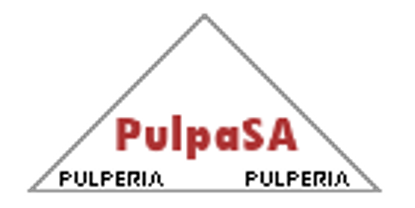
\includegraphics[width=0.5\textwidth]{images/image.png} 
    %\vspace{2cm}

    {\Huge \textbf{\thetitle}} \\[1cm]
    {\large Game Design Document} \\[1.5cm]

    \vspace*{\fill}

    {\large \textbf{\theauthor}} \\ [1cm]
    {\large IES San Clemente} \\[4cm]

    \vspace*{\fill} % Empuja hacia la parte inferior

    {\large \today}

    \restoregeometry % Restaura los márgenes normales para el resto del documento
\end{titlepage}



\renewcommand{\contentsname}{Índice}

\tableofcontents

% start sections by 1

\newpage

\section{Pitch}

\subsection{Visión xeral do xogo}
PulpaSA é un videoxogo de xestión para PC inspirado en Overcooked. Está 
ambientado na romaría galega, onde o xogador ou xogadores tomarán o rol de 
traballadores dunha pulpería ambulante, a cal sirve a comensais durante o 
transcurso dunha romaría tradicional galega, onde se enfrontarán ao frenético 
reto de satisfacer a demanda da clientela.

\subsection{Concepto do xogo}

Cada nivel estará ambientado nunha festa/romaría dunha vila Galega. O 
escenario (o posto ambulante, tamén coñecido como “carro do polbo”) será 
sempre o mesmo, coa diferencia de que en cada festa (nivel) tentarase 
mostrar elementos que distingan a vila onde se está desenvolvendo a festa. A 
dificultade do xogo podería adecuarse en función da afluencia e fama de dita 
romaría ou festa. O estilo visual será “Cartoon”.

%image
\begin{figure}[h]
    \centering
    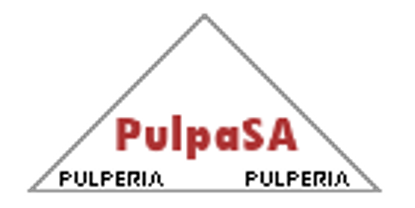
\includegraphics[width=0.2\textwidth]{images/pulpasa_logo.png}
    \caption{Logo PulpaSA}
    \label{fig:Boceto Logo PulpaSA}
\end{figure}

\begin{figure}[h]
    \centering
    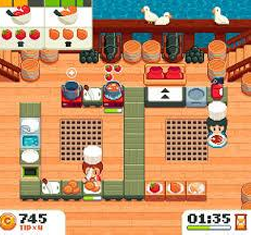
\includegraphics[width=0.5\textwidth]{images/concept_game.png}
    \caption{Captura conceptual PulpaSA}
    \label{fig:Captura conceptual PulpaSA}
\end{figure}

\newpage

\subsection{Mecánica principal}
O xogador ou xogadores deberán atender as comandas da clientela, nas cales, 
o produto principal sempre será o polbo, onde o cliente poderá demandar una 
condimentación específica (pimentón doce ou picante), sal (nada, pouco, 
normal, e moito), cachelos (si ou non), e aceite (nada, pouco, normal e moito). 
O xogo estaría pensado para mínimo 2 persoas en multixogador local, ou 
posibilidade de modo Individual, onde o xogador tomará o control de 2 NPC’s 
cos cales, de forma simultánea, tería que asumir todas as tarefas. No caso de 
2 xogadores, os roles asúmense a gusto dos xogadores, e deberán 
coordinarse e traballar en equipo para conseguir servir as comandas a tempo. 

\subsubsection{Tarefas}
\begin{itemize}
    \item Cortar (Tanto cachelos como polbo)
    \item Cocer (estar atento a cocción)
    \item Lavar pratos
    \item Condimentar co nivel solicitado polo cliente (Sal, Pimentón e Aceite)
    \item Servir a comanda na sección da mesa que corresponda (Pratos, bebidas
    e pan)
\end{itemize}

\subsection{Mercado obxectivo}

\subsubsection{Público}
Xogadores de todo tipo (experimentados e casuais) de calquera franxa de 
idade que estean interesados en xogos cooperativos. 

\subsubsection{Posicionamento no mercado}
Overcooked é un xogo moi afamado que, pese ao paso do tempo, sigue 
mantendo xogadores. PulpaSA diferenciaríase de Overcooked ao ofrecer un 
enfoque cultural único e, unha mecánica de xogo máis simple, ao reducir as 
elaboración culinarias ao contexto das pulperías en romarías galegas. 

\subsection{Equipo e capacidades}

PulpaSA estará desenvolto por una persoa únicamente

\subsection{Plan de desarrollo}

Os prazos están definidos polo profesorado. O obxectivo será crear un MVP 
abarcable para os tempos establecidos (un único nivel de cara a DEMO, modos 
un xogador e multixogador local (multixogador en liña se o tempo o permite)). 
\begin{itemize}
    \item \textbf{Febreiro-Marzo:} Creación / escoller deseños recursos gráficos, comezar coas 
primeiras escenas do xogo (Escena Menú principal, Escena do primeiro nivel, e 
prototipo inicial) 
\item \textbf{Abril-Maio:} Implementar lóxica/funcionalidade e son 
\item \textbf{Xuño:} Testing e corrección de erros 
\end{itemize}

\subsection{Hook único}
Pese a que as mecánicas desta proposta son coñecidas (mixturar cooperación 
co caos que pode ser xestionar un negocio gastronómico), o que diferencia a 
PulpaSA das alternativas do mercado é o seu enfoque cultural único e 
inmersivo nas tradicións galegas. A ambientación nas romarías, os desafíos 
específicos como a preparación do polbo á galega, e os detalles humorísticos 
inspirados no folclore local crean unha experiencia que combina diversión e 
autenticidade. PulpaSA non só invita aos xogadores a divertirse, senón tamén a 
descubrir e celebrar a riqueza da gastronomía e das festas populares galegas, 
ofrecendo unha aventura que destaca pola súa identidade propia nun mercado 
globalizado.

\section{Game Concept}

\subsection{Temática}
PulpaSA está ambientado nas tradicionais romarías galegas, ofrecendo unha 
experiencia única que celebra as costumes locais. O xogador mergúllase no 
vibrante ambiente dunha pulpería ambulante, enfrontándose ao desafío 
frenético de atender aos comensais con precisión e rapidez. Os piares do xogo 
xiran arredor da cooperación, o caos controlado e unha inmersión cultural que 
destaca a riqueza das tradicións gastronómicas e festivas de Galicia. 

\subsection{Xénero}
PulpaSA clasifícase como un xogo de xestión e cooperación, inspirado nas 
dinámicas de títulos como Overcooked. En termos de subxéneros, pertence 
aos xogos de estratexia en tempo real, cun enfoque en tarefas culinarias, 
traballo en equipo e coordinación. 

\subsection{Estilo visual}
Inicialmente, no GamePitch planteeino en “Pixel art”, pero despois de meditalo, 
prefiro un estilo visual en 3D cartoon, con gráficos coloridos. A cámara terá un 
punto de vista cenital, similar ao utilizado en Overcooked, o que permitirá aos 
xogadores visualizar claramente o entorno completo do posto ambulante e as 
áreas de interacción. 

\subsection{Mockups pantallas}
\begin{figure}[h]
    \centering
    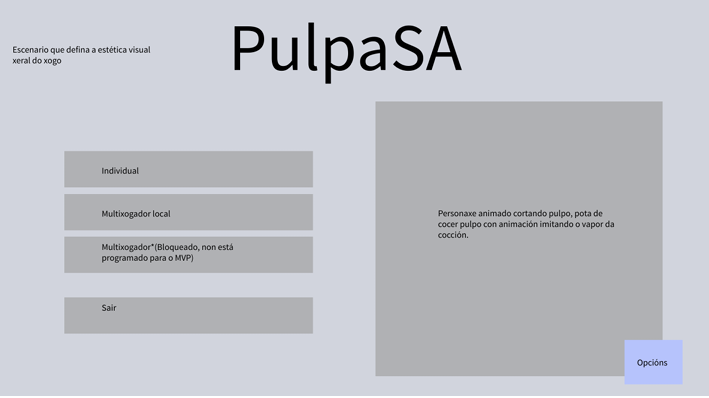
\includegraphics[width=1\textwidth]{images/mockup1.png}
    \caption{Mockup Pantalla Principal}
    \label{fig:Mockup Pantalla Principal}
\end{figure}

%seleccion niveles

\begin{figure}[h]
    \centering
    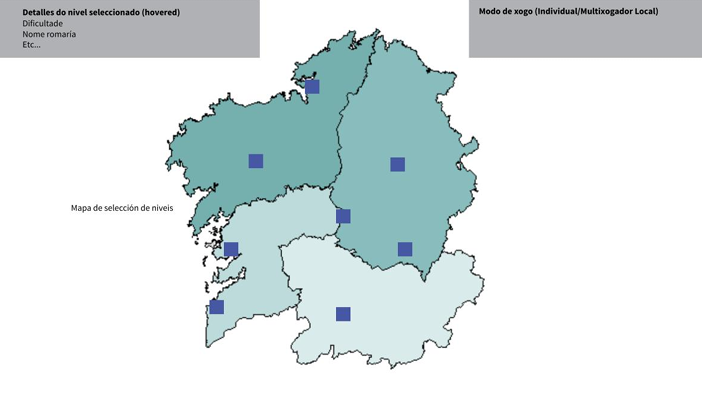
\includegraphics[width=1\textwidth]{images/mockup2.png}
    \caption{Mockup Selección de Niveles}
    \label{fig:Mockup Selección de Niveles}
\end{figure}

%escena de xogo

\begin{figure}[h]
    \centering
    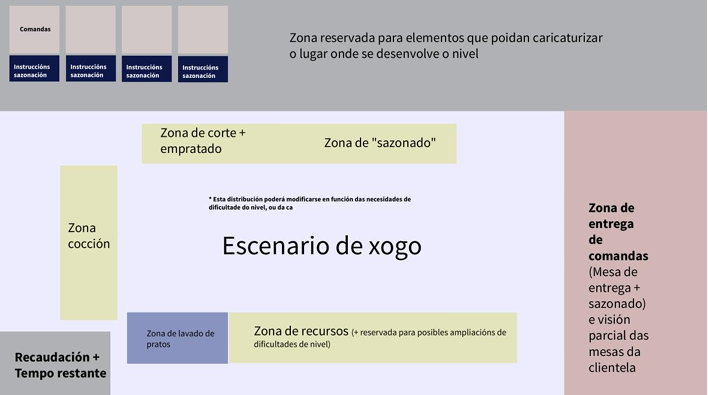
\includegraphics[width=1\textwidth]{images/mockup3.png}
    \caption{Mockup Escena de Xogo}
    \label{fig:Mockup Escena de Xogo}
\end{figure}

\clearpage
\subsection{Inspiración}

\subsubsection{Proposta 1}
O estilo visual desta UI axeitase bastante a estética que busco para PulpaSA, 
adaptando os elementos decorativos e cambiandoos por visuais propios do 
lore que vamos a tratar (Toldo branco, a madeira (xa está), o polbo, e os pratos 
de madeira característicos), creo que podería funcionar .
\begin{figure}[h]
    \centering
    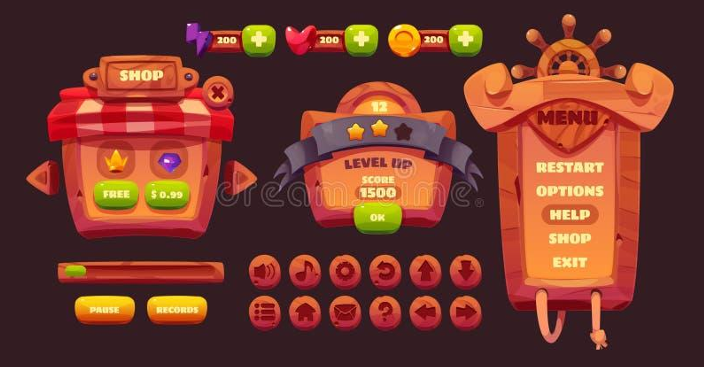
\includegraphics[width=1\textwidth]{images/inspiracion1.png}
    \caption{Deseño de UI}
    \label{fig:Overcooked}
\end{figure}
\clearpage
\subsubsection{Proposta 2}
Moi simple en canto a elementos visuais, o que máis me chama a atención é o 
minimalismo (totalmente o oposto ao primeiro exemplo).
\begin{figure}[h]
    \centering
    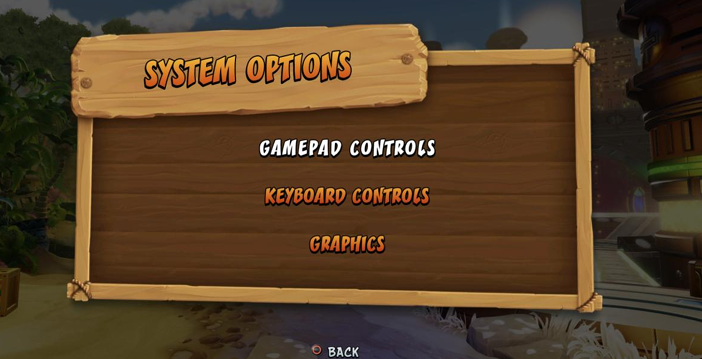
\includegraphics[width=1\textwidth]{images/inspiracion2.png}
    \caption{Snapshot Crash Bandicoot}
    \label{fig:Proposta ui (Crash Bandicoot)}
\end{figure}
\clearpage
\subsubsection{Proposta 3}
Pareceume curiosa o arte de este mapa 2D (mapa e lenda), nun xogo que, en 
gameplay, ten unha estética muy similar ao que busco. 

\begin{figure}[h]
    \centering
    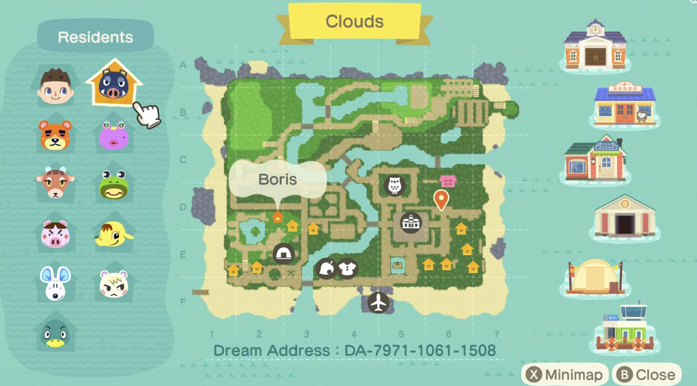
\includegraphics[width=1\textwidth]{images/inspiracion3.png}
    \caption{Snapshot Animal Crossing}
    \label{fig:Snapshot Animal Crossing}
\end{figure}
\clearpage
\subsubsection{Proposta 4}
Simplicidade comparable a segunda captura (Crash Bandicoot), pero con unha 
estética máis similar ao que busco (Cartoon)
\begin{figure}[h]
    \centering
    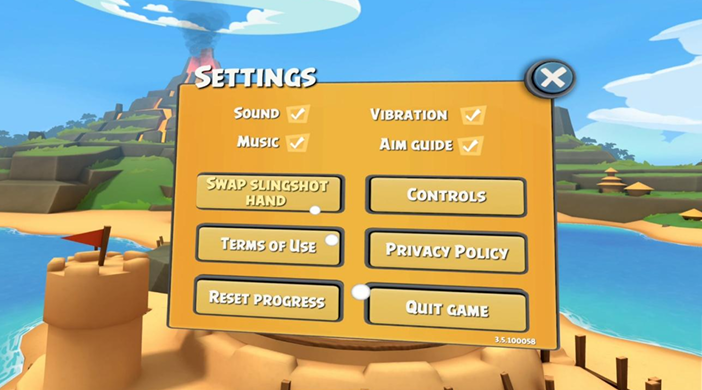
\includegraphics[width=1\textwidth]{images/inspiracion4.png}
    \caption{Snapshot UI}
    \label{fig:Snapshot}
\end{figure}


\clearpage


\section{Mecánicas}

\begin{table}[h]
    \centering
    \renewcommand{\arraystretch}{1.3} % Aumenta la altura de las filas
    \setlength{\tabcolsep}{10pt} % Espaciado entre columnas
    \label{tab:mecanicas}
    \rowcolors{2}{gray!15}{white} % Colores alternos en las filas
    \begin{tabular}{|p{4cm}|p{2cm}|p{3cm}|p{4cm}|}
        \hline
        \rowcolor{octopus} % Color de fondo para la fila del encabezado
        \textbf{Mecánica}  & \textbf{Tipo} & \textbf{Necesidad} & \textbf{Reglas} \\
        \hline
        Atender Comandas & Primaria  & Interaccion con obxectos  & Os xogadores deben xestionar pedidos de clientes \\
        \hline
        Coordinación cooperativa & Primaria  & Multixogador    & Se permite atacar enemigos con un arma o golpe cuerpo a cuerpo. \\
        \hline
        Preparación de ingredientes  & Secundaria & Interacción con obxectos & Cortar cachelos/polbo antes de cocelos \\
        \hline
        Cocción & Secundaria & Xestión do transcurso do tempo / FSM & Estar pendente da cocción dos ingredientes \\
        \hline
        Condimentación & Secundaria & Interacción con obxectos & Engadir sal, pementa, aceite, etc. \\
        \hline
        Limpeza de pratos & Secundaria & Interacción con obxectos & Limpar cando se esgoten \\
        \hline
        Variación de dificultade  & Sistema & Xestión de dificultade & Aumento da demanda de comandas \\
        \hline
        Valoración de comandas & Sistema & Xestión de puntuación & Puntuación en función da satisfacción do cliente \\
        \hline

    \end{tabular}
    %\caption{Táboa de Mecánicas}
\end{table}

\newpage
\section{Narrativa}

Pese a que PulpaSA é un xogo plenamente de xestión, tentarase darlle un contexto histórico sinxelo con un toque humorístico.

\subsection{Idea}

Videoxogo de xestión cooperativa dunha pulpería ambulante, onde cada nivel correspondería a unha romería galega.

\subsection{Logline}

Os xogadores traballan nunha pulpería ambulante durante unha romaría galega, onde deben coordinarse para servir pratos de polbo baixo presión.

\subsection{Sipnose}

Un grupo de amigos norteamericanos, que orixinariamente traballaban arreo nunha consultoría de software, e eran víctimas do burnout, deciden
abandonar todo e montar unha pulpería moi influenciada pola cultura Fast-Food americana, coa que percorrerán toda a xeografía galega en busca de romarías onde poidan ir acadando boa fama.
 Todo isto ocorre despois de que o grupo viñese de vacacións a Galicia, e quedasen ledos coa cultura
e tradición. A idea de montar unha pulpería ambulante xurdiu nunha noite de copas, e aínda que ao principio parecía unha idea disparatada,
acabou por materializarse. O inicio non será fácil... pero coa tua axuda, poderán conseguilo!

\subsection{Arquetipo}

PulpaSA toma como referencia o arquetipo do heroe:
%listar arquetipos
\begin{itemize}
    \item \textbf{O heroe}: Os protagonistas deciden abrir a pulpería
    \item \textbf{Desafíos iniciais}: Aprender a xestionar a pulpería
    \item \textbf{Complicacións}: Incrementase cada vez máis a demanda / complexidade dos pedidos
    \item \textbf{Clímax}: A pulpería logra acadar os obxectivos mínimos
    \item \textbf{Resolución}: PulpaSA é un éxito
\end{itemize}

\subsection{Estrutura Narrativa}

O xogo, en canto a estrutura narrativa, dividirase en 3 seccións claramente diferenciadas (introducción, nudo e desenlace):

\begin{itemize}
    \item \textbf{Inicio}: Introdución ao xogo, pequena animación onde se presenta o contexto do xogo e se ensinan as mecánicas clave.
    \item \textbf{Nudo}: Cada un dos niveis que o xogador terá que superar
    \item \textbf{Desenlace}: Animación final onde se caricaturiza o éxito (ou quizáis o fracaso) da pulpería
\end{itemize}


\newpage
\section{Personaxes}
O xogo, nun escenario ideal, contaría con 4 personaxes xogables a elexir,

\subsection{Personaxe 1}
\subsubsection{Nombre}
John Cea
\subsubsection{Importancia en el Juego}
Socio fundador de PulpaSA \footnotemark[1]
\subsubsection{Rasgos característicos}
Ten a capacidade de limpar os pratos máis rápido \footnotemark[2]
\subsubsection{Transformación}
Os personaxes non teñen unha transformación, dado que é un xogo de xestión, onde prima a habilidade e rapidez dos xogadores.

\subsection{Personaxe 2}
\subsubsection{Nombre}
Bill Gatos
\subsubsection{Importancia en el Juego}
Socio fundador de PulpaSA \footnotemark[1]
\subsubsection{Rasgos característicos}
Ten a capacidade de cortar os ingredientes máis rápido \footnotemark[2]
\subsubsection{Transformación}
Os personaxes non teñen unha transformación, dado que é un xogo de xestión, onde prima a habilidade e rapidez dos xogadores.


\subsection{Personaxe 3}
\subsubsection{Nombre}
Vanessa Poconcho
\subsubsection{Importancia en el Juego}
Socio fundador de PulpaSA \footnotemark[1]

\subsubsection{Rasgos característicos}
Ten a capacidade de cocer os ingredientes máis rápido \footnotemark[2]
\subsubsection{Transformación}
Os personaxes non teñen unha transformación, dado que é un xogo de xestión, onde prima a habilidade e rapidez dos xogadores.


\subsection{Personaxe 4}
\subsubsection{Nombre}
Natalie Newport
\subsubsection{Importancia en el Juego}
Socio fundador de PulpaSA \footnotemark[1]
\subsubsection{Rasgos característicos}
Ten a capacidade de condimentar con 2 condimentos na mesma acción \footnotemark[2]
\subsubsection{Transformación}
Os personaxes non teñen unha transformación, dado que é un xogo de xestión, onde prima a habilidade e rapidez dos xogadores.

\footnotetext[1]{Todos os personaxes teñen a mesma relevancia no xogo.}
\footnotetext[2]{As habilidades poderán mudar durante a fase de probas, co obxectivo de equilibrar a dificultade.}

\newpage
\section{Deseño de nivel DEMO}
\subsection{Boceto}
Estrutura semiaberta con zonas de interacción divididas por función (corte, preparacion, entrega,...). O escenario
será un campo de terra con céspede, cuxo entorno decoraráse con elementos característicos duna romaría ou festa.

\subsubsection{Burbullas ou etapas do nivel}
\begin{itemize}
    \item \textbf{Zona de preparación}: Mesas para cortar ingredientes (pulpo ou cachelos)
    \item \textbf{Zona de cocción}: Olla para cocer os ingredientes
    \item \textbf{Zona de preparación e entrega}: Aplicar especiado no nivel requerido pola comanda e entregar a cliente
    \item \textbf{Zona de almacenamento}: Espazo para almacenar os ingredientes básicos (cachelos, polbo, sal, aceite, pimentón)
    \item \textbf{Eventos de entorno}: Interrupcións externas (por exemplo, un grupo de gaiteiros que pasan pola zona de preparación)
\end{itemize}
\subsubsection{Obxectivos}

% taboa de obxectivos e detalle do obxectivo

\begin{table}[h]
    \centering
    \renewcommand{\arraystretch}{1.3} % Aumenta la altura de las filas
    \setlength{\tabcolsep}{10pt} % Espaciado entre columnas
    \label{tab:obxectivos}
    \rowcolors{2}{gray!15}{white} % Colores alternos en las filas
    \begin{tabular}{|p{4cm}|p{9cm}|}
        \hline
        \rowcolor{octopus} % Color de fondo para la fila del encabezado
        \textbf{Obxectivo}  & \textbf{Detalle} \\
        \hline
        Servir o obxectivo de comandas no prazo requerido & As comandas serán o resultado da ausencia presencia de cachelos, patacas, pementou ou sal \\
        \hline
        Introducir Mecánicas básicas & O xogador deberá aprender a cortar, cocer e condimentar os ingredientes \\
        \hline
        Coordinarse (cooperativo) & O xogador deberá coordinarse co resto de xogadores para conseguir o obxectivo \\
        \hline
    \end{tabular}
    \caption{Táboa de Obxectivos}
\end{table}

\subsubsection{Obstáculos}

\begin{table}[h]
    \centering
    \renewcommand{\arraystretch}{1.3} % Aumenta la altura de las filas
    \setlength{\tabcolsep}{10pt} % Espaciado entre columnas
    \label{tab:obstaculos}
    \rowcolors{2}{gray!15}{white} % Colores alternos en las filas
    \begin{tabular}{|p{4cm}|p{9cm}|}
        \hline
        \rowcolor{octopus} % Color de fondo para la fila del encabezado
        \textbf{Obstáculo}  & \textbf{Detalle} \\
        \hline
        Terreo irregular & Algunhas zonas poden ter barro e o personaxe podería esvarar \\
        \hline
        Paciencia Cliente & Debaixo de cada comanda, aleatoriamente poderíase activar un timeout que indicaria a paciencia do cliente (tempo de espera) \\
        \hline
    \end{tabular}
    \caption{Táboa de Obstáculos}
\end{table}

\clearpage

\subsubsection{Elementos de ambiente/script}
% taboa de elementos de ambiente e script
\begin{table}[h]
    \centering
    \renewcommand{\arraystretch}{1.3} % Aumenta la altura de las filas
    \setlength{\tabcolsep}{10pt} % Espaciado entre columnas
    \label{tab:elementos}
    \rowcolors{2}{gray!15}{white} % Colores alternos en las filas
    \begin{tabular}{|p{4cm}|p{9cm}|}
        \hline
        \rowcolor{octopus} % Color de fondo para la fila del encabezado
        \textbf{Elemento}  & \textbf{Detalle} \\
        \hline
        Obxectos interactivos & Mesas, cociña, ollas, pratos, etc. \\
        \hline
        Personaxes NPC & Clientes que demandan comida e que se van marchando cando non son atendidos \\
        \hline
        Cliente Impaciente & Cliente que se marcha sen ser atendido porque se lle esgota a paciencia \\
        \hline
        Son ambiental & Son ambiental que aporte atmósfera \\
        \hline
    \end{tabular}
    \caption{Táboa de Elementos de ambiente}
\end{table}



\subsection{Características de nivel}

\subsubsection{Estética visual festa tradicional mezclada co mundo moderno}
O nivel estará ambientado nunha romaría tradicional galega, onde se os elementos visuais predominantes no 
entorno serán elementos típicos de romarías (carrozas, gaiteiros, etc.). O que romperá por completo esta estetica é o posto ambulante, que será un carro de polbo, pero cunha estética moderna e minimalista.

\subsubsection{Xogabilidade caótica}
A xogabilidade será frenética, onde os xogadores deberán coordinarse para atender as comandas dos clientes, mentres que a presión aumentará a medida que o tempo pase. O obxectivo é servir as comandas antes de que os clientes se marchen.

\subsubsection{Conflicto entre o gremio tradicional e a pulpería moderna}
O nivel representa unha tensión simbólica entre os pulpeiros tradicionais e a nova pulpería moderna enfocada na produción masiva. Mentres os primeiros defenden a autenticidade, o saber facer herdado e o respecto polos tempos da cocción artesanal, a pulpería moderna aposta pola eficiencia, a marca e a estetización do produto.

\newpage
\subsection{Referencias visuais}
\begin{figure}[h]
    \centering
    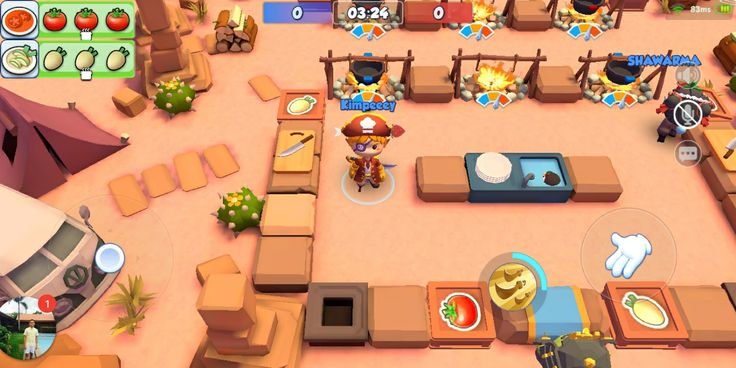
\includegraphics[width=0.8\textwidth]{images/overcooked_concept.jpg}
    \caption{Snapshot Overcooked exterior}
    \label{fig:Snapshot Overcooked exterior}
\end{figure}

\begin{figure}[h]
    \centering
    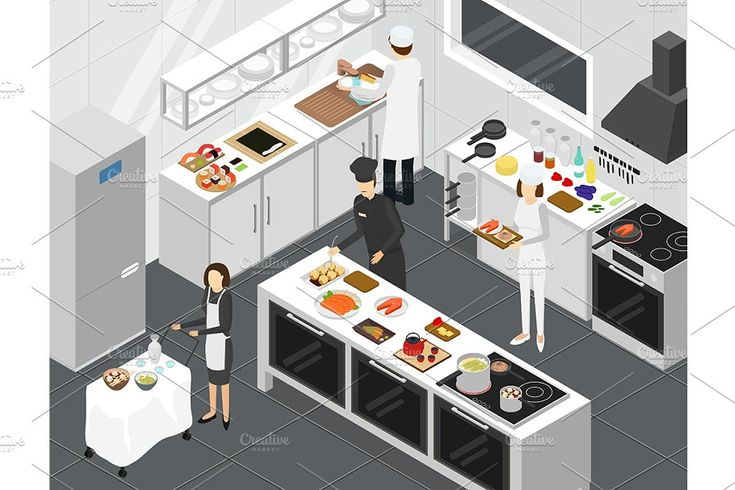
\includegraphics[width=0.9\textwidth]{images/kitchen_furniture_concept.jpg}
    \caption{Concepto de moblaxe de cociña}
    \label{fig:Snapshot Overcooked}
\end{figure}

\begin{figure}[h]
    \centering
    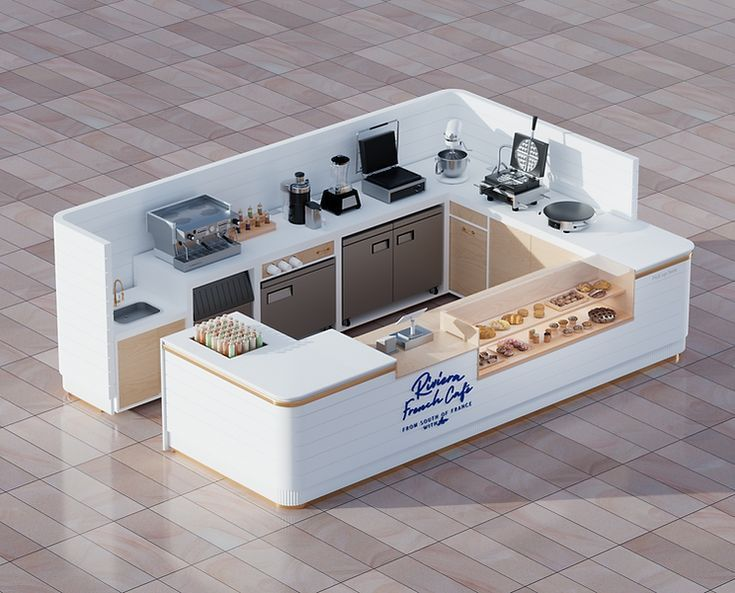
\includegraphics[width=0.9\textwidth]{images/kitchen_furniture_concept_1.jpg}
    \caption{Modelo de moblaxe de cociña}
    \label{fig:Modelo de moblaxe de cociña}
\end{figure}

\clearpage


\subsection{Elementos}

\begin{table}[h]
    \centering
    \renewcommand{\arraystretch}{1.3}
    \setlength{\tabcolsep}{10pt}
    \label{tab:assets}
    \rowcolors{2}{gray!15}{white}
    \begin{tabular}{|p{4cm}|p{9cm}|}
        \hline
        \rowcolor{octopus}
        \textbf{Asset} & \textbf{Descripción} \\
        \hline
        Posto de pulpería moderno & Estructura modular de estilo híbrido tradicional/moderno. \\
        \hline
        Caldeiro de cobre & Utensilio clásico para cocción con animaciones. \\
        \hline
        Packaging pedidos & Presentación moderna con diseño corporativo. \\
        \hline
        Estación preparado de pedido & Mesa onde se introduce o producto dentro do packaging \\
        \hline
        Decoración entorno romaría & Alguns elementos decorativos que den ambientación de romaría \\
        \hline
        Chan e entorno & Chan de terra con céspede e zonas de paso dificultoso (barro) \\
        \hline
        Ingredientes principais & Polbo, cachelos, sal, aceite e pimentón \\
        \hline
    \end{tabular}
    \caption{Assets a desarrollar}
\end{table}

% taboa de elementos de UI
\begin{table}[h]
    \centering
    \renewcommand{\arraystretch}{1.3} % Aumenta la altura de las filas
    \setlength{\tabcolsep}{10pt} % Espaciado entre columnas
    \label{tab:ui}
    \rowcolors{2}{gray!15}{white} % Colores alternos en las filas
    \begin{tabular}{|p{4cm}|p{9cm}|}
        \hline
        \rowcolor{octopus} % Color de fondo para la fila del encabezado
        \textbf{Elemento}  & \textbf{Descripción} \\
        \hline
        Barra de tempo & Indicador do tempo restante para servir a comanda \\
        \hline
        Iconos de ingredientes & Iconos para construir os tickets de comandas \\
        \hline
        Deseño de UI & Estilo visual do menú principal e selección de nivel \\
        \hline
    \end{tabular}
    \caption{Assets UI}
\end{table}

% taboa personaxes

\begin{table}[h]
    \centering
    \renewcommand{\arraystretch}{1.3} % Aumenta la altura de las filas
    \setlength{\tabcolsep}{10pt} % Espaciado entre columnas
    \label{tab:personaxes}
    \rowcolors{2}{gray!15}{white} % Colores alternos en las filas
    \begin{tabular}{|p{4cm}|p{9cm}|}
        \hline
        \rowcolor{octopus} % Color de fondo para la fila del encabezado
        \textbf{Personaxe}  & \textbf{Descripción} \\
        \hline
        Personaxe 1 & Personaxe xogable 1 (John Cea) \\
        \hline
        Personaxe 2 & Personaxe xogable 2 (Bill Gatos) \\
        \hline
        Personaxe 3 & Personaxe xogable 3 (Vanessa Poconcho) \\
        \hline
        Personaxe 4 & Personaxe xogable 4 (Natalie Newport) \\
        \hline
        Personaxe NPC & Personaxe non xogable (Cliente) \\
        \hline
    \end{tabular}
    \caption{Assets Personaxes}
\end{table}

\newpage
\subsection{Música}
% tabla clasificada por familias, DX, MX, FOL y BG

\begin{table}[h]
    \centering
    \renewcommand{\arraystretch}{1.3} % Aumenta la altura de las filas
    \setlength{\tabcolsep}{10pt} % Espaciado entre columnas
    \label{tab:muxica}
    \rowcolors{2}{gray!15}{white} % Colores alternos en las filas
    \begin{tabular}{|p{4cm}|p{9cm}|}
        \hline
        \rowcolor{octopus} % Color de fondo para la fila del encabezado
        \textbf{Familia}  & \textbf{Descripción} \\
        \hline
        FOL & Ruido fondo romaría \\
        \hline
        BG & Música de fondo \\
        \hline
        FX & Efectos de son (corte, cocción, etc.) \\
        \hline
        FX & Efectos de son (interacción con obxectos) \\
        \hline
        FX & Efectos de son (Entrega de pedido e nova comanda) \\
        \hline
    \end{tabular}
    \caption{Música e efectos}
\end{table}

\end{document}
